% #############################################################################
% Appendix B - Microfluidics Internship
% !TEX root = ../main.tex
% #############################################################################

\fancychapter{Microfluidics Internship}
\label{appendix:b}

This appendix presents the microfluidics internship conducted in parallel with the development of this thesis. Both the \ac{MR} sensors and microfluidic channels utilized in this application were fabricated at \ac{INESC-MN}. During the internship, I had the valuable opportunity to observe and engage in a portion of the microfluidic channel fabrication process. This firsthand experience provided valuable insights and complemented the development of the interface, enhancing the overall understanding and integration of the project.

\begin{figure}[!ht]
    \centering
    \begin{subfigure}[b]{.475\linewidth}
        \centering
        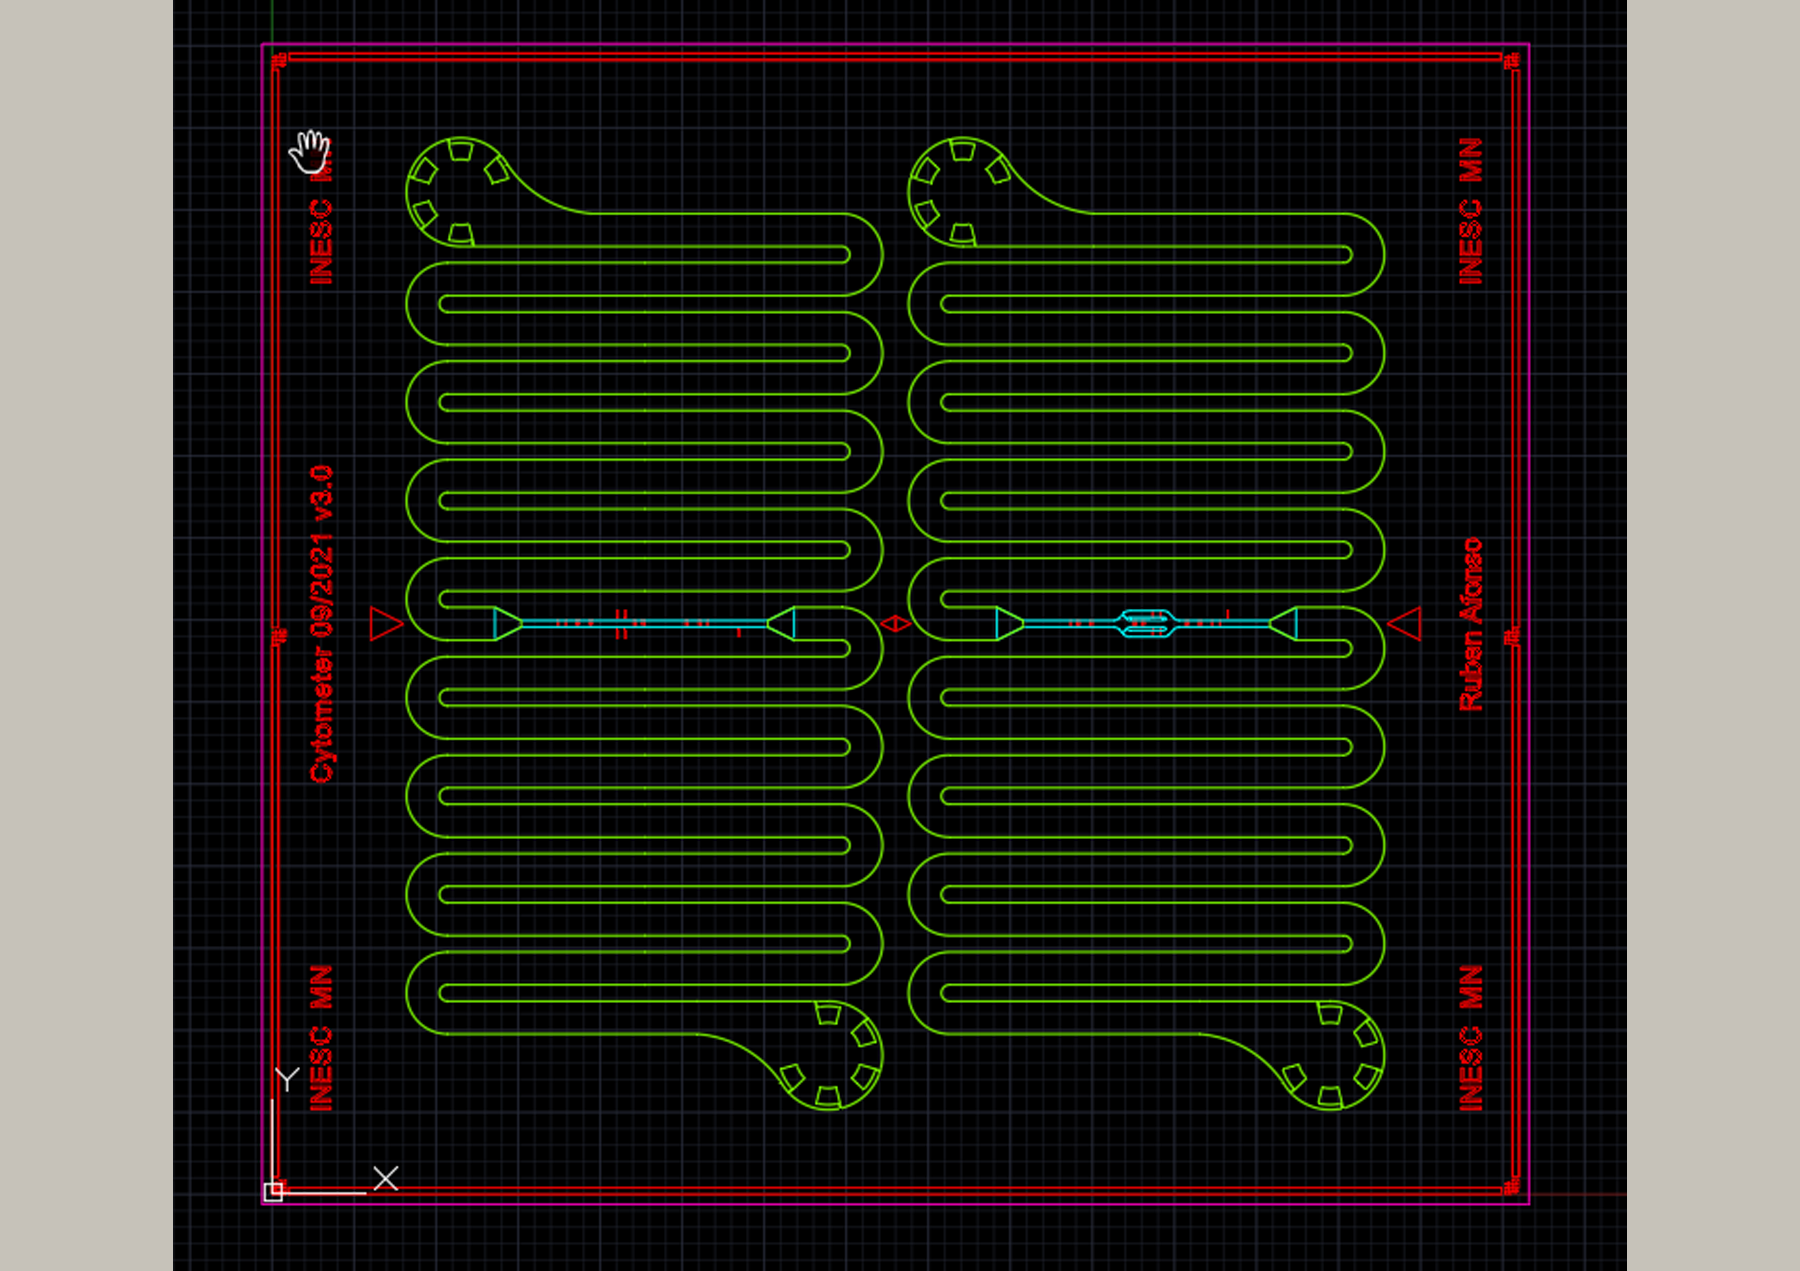
\includegraphics[width=\linewidth]{images/appendix_b/mask.png}
        \caption{Mask -- developed by Eng. Ruben Afonso.}
        \label{figure:pdms-mask}
    \end{subfigure}
    \hfill
    \centering
    \begin{subfigure}[b]{.475\linewidth}
        \centering
        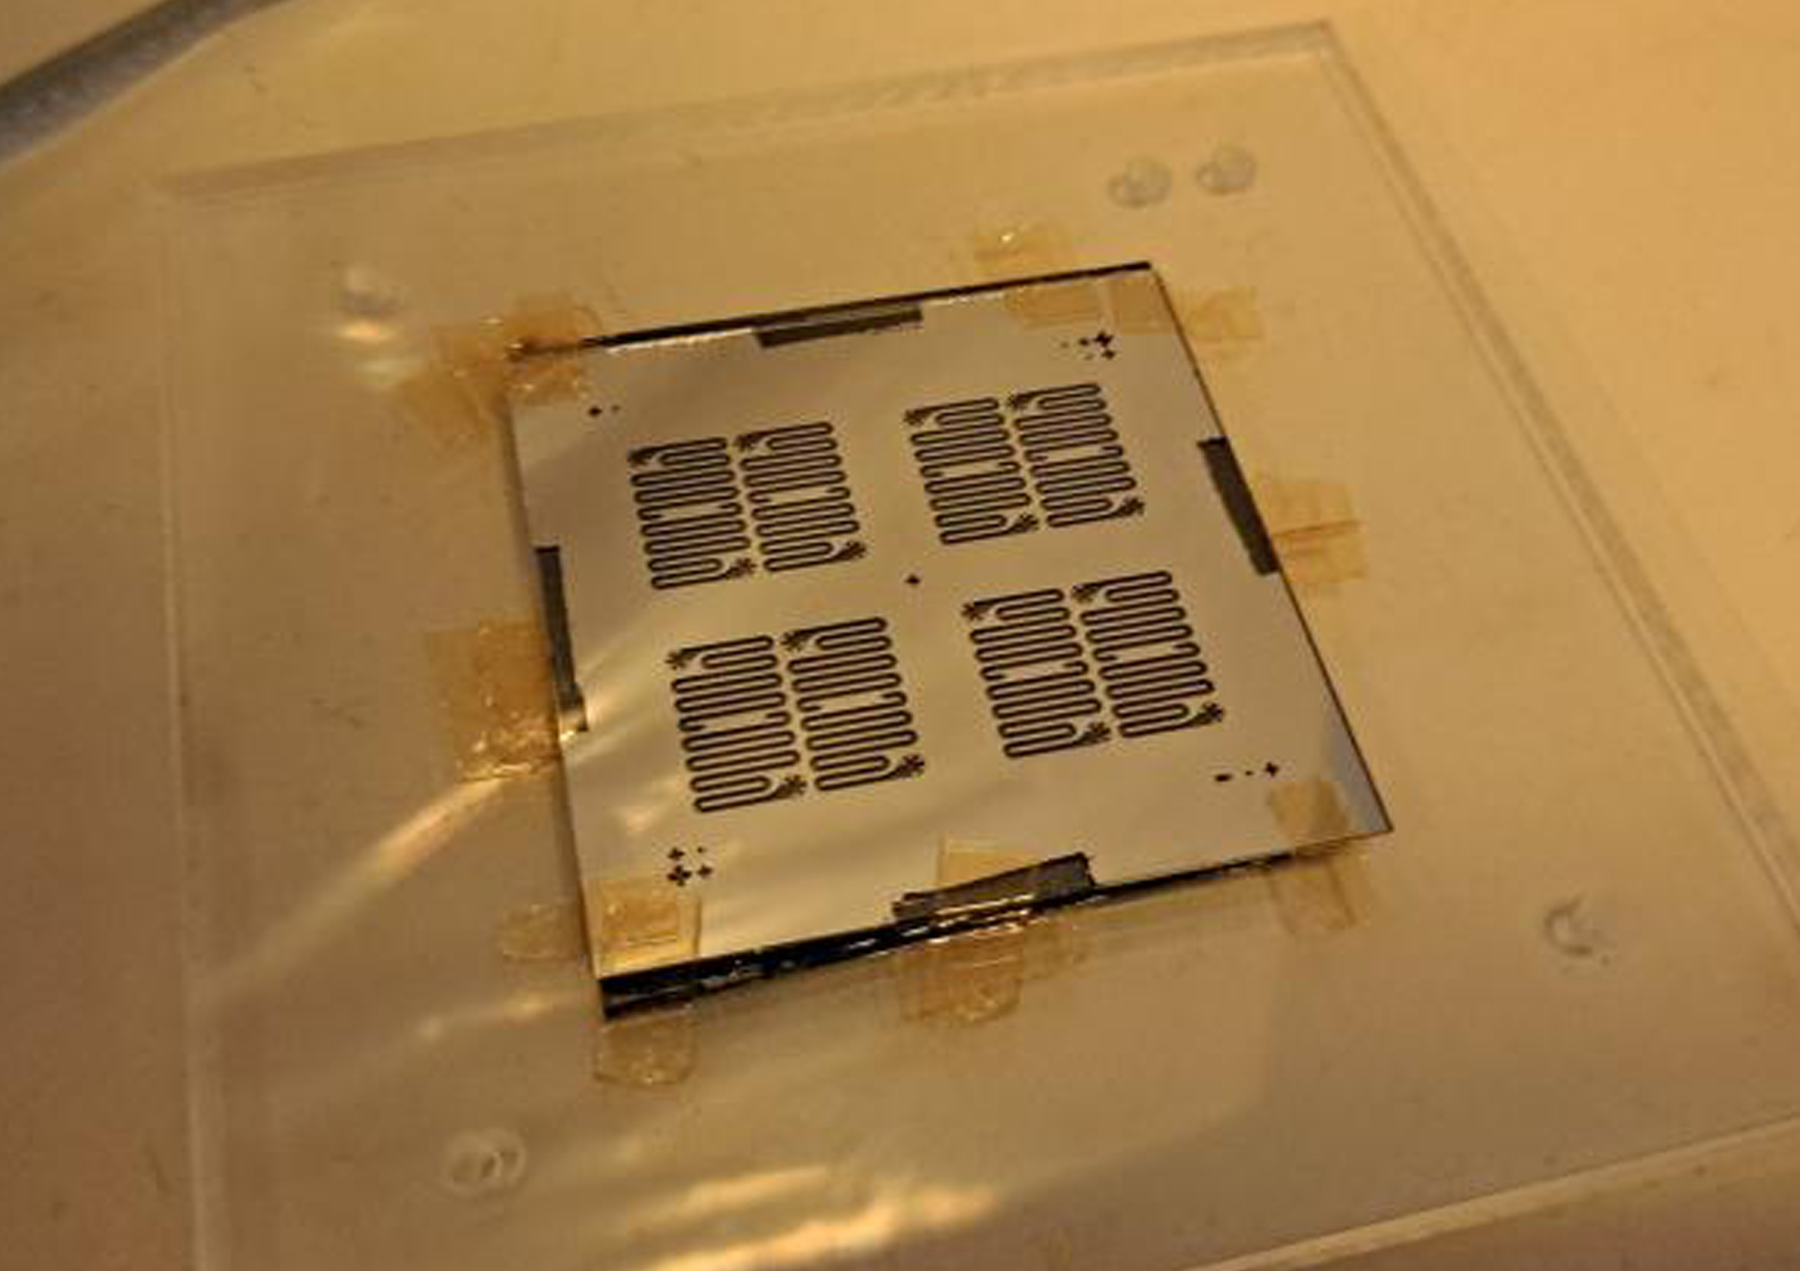
\includegraphics[width=\linewidth]{images/appendix_b/hardmask.png}
        \caption{Hard-mask}
        \label{figure:pdms-hardmask}
    \end{subfigure}

    \bigskip
    
    \centering
    \begin{subfigure}[b]{.475\linewidth}
        \centering
        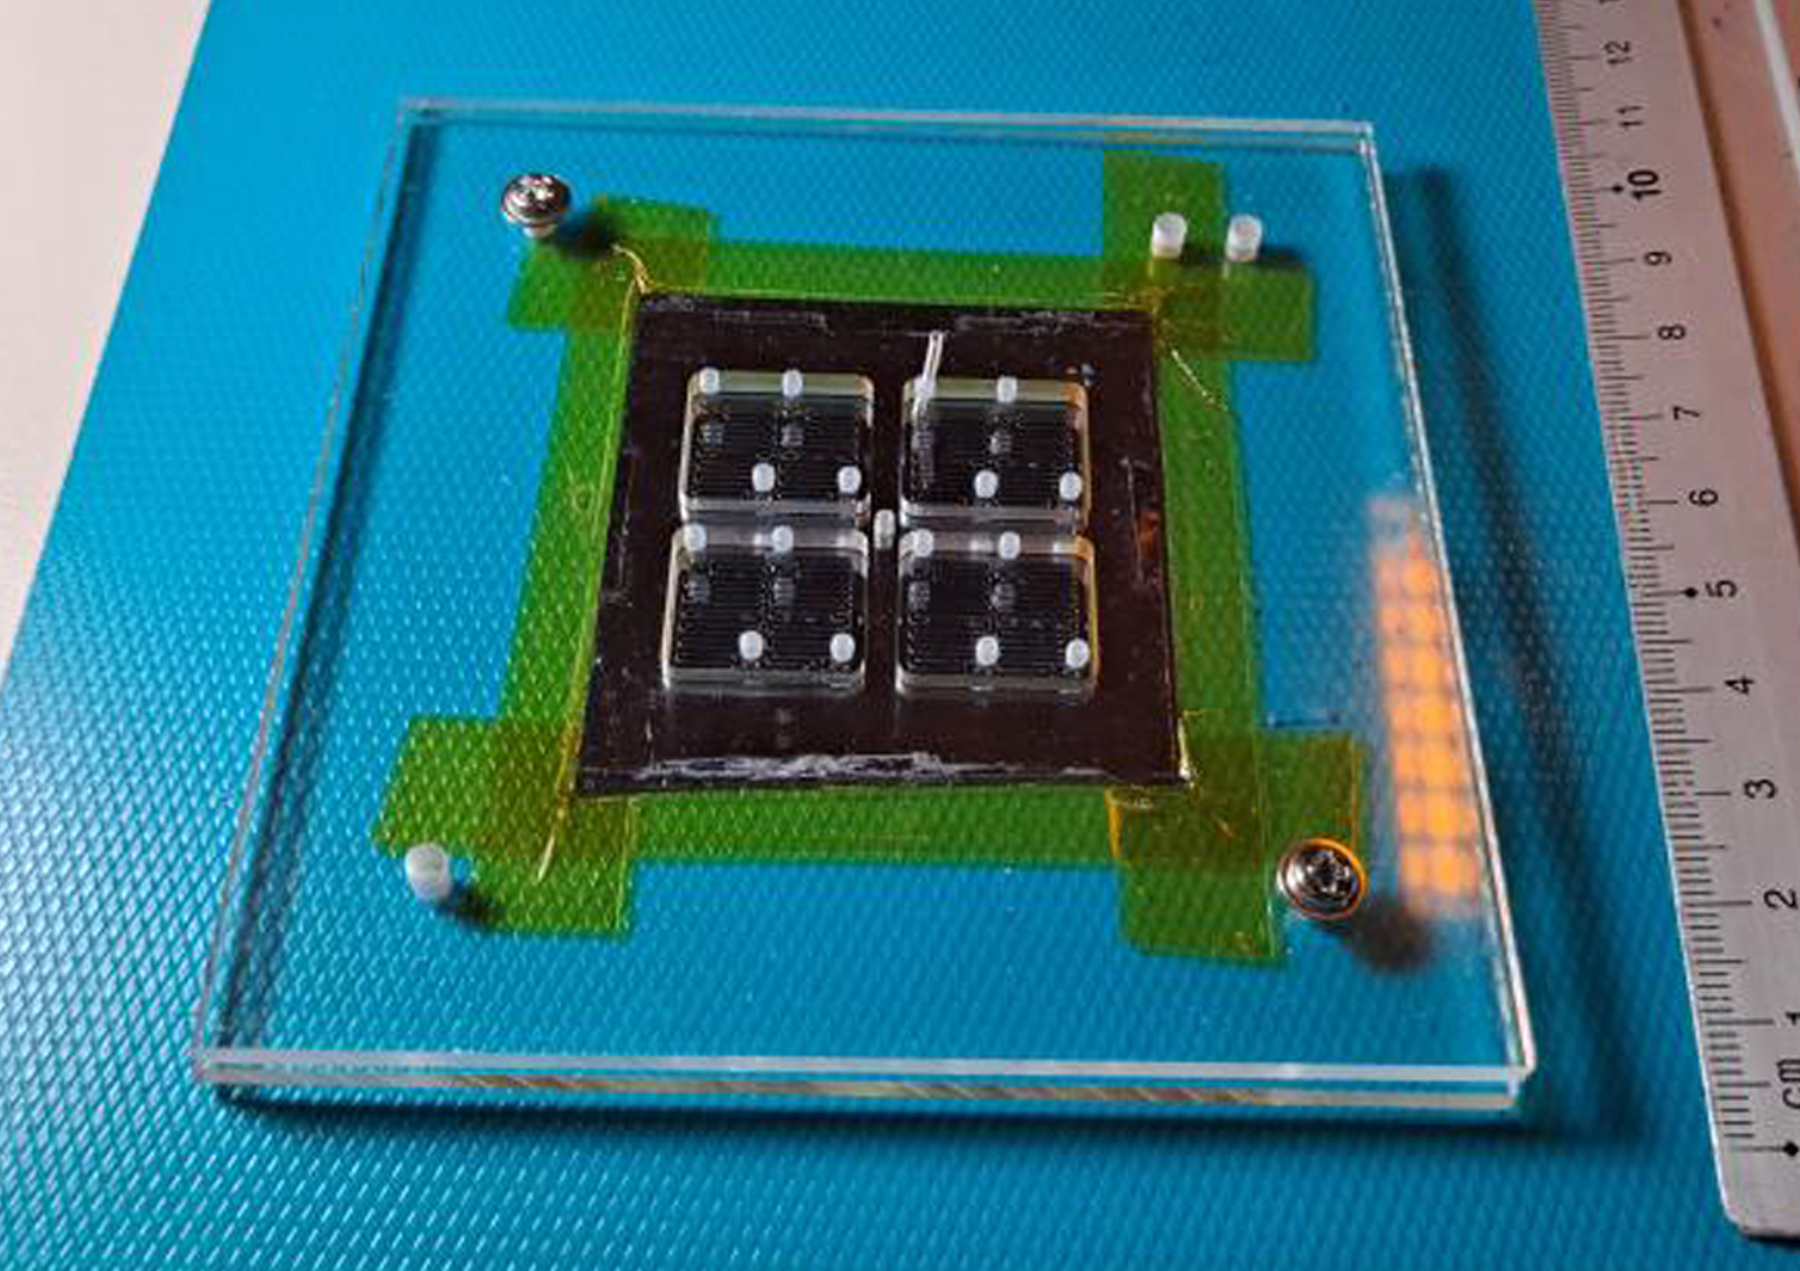
\includegraphics[width=\linewidth]{images/appendix_b/mold.png}
        \caption{Acrilic mold.}
        \label{figure:pdms-mold}
    \end{subfigure}
    \hfill
    \centering
    \begin{subfigure}[b]{.475\linewidth}
        \centering
        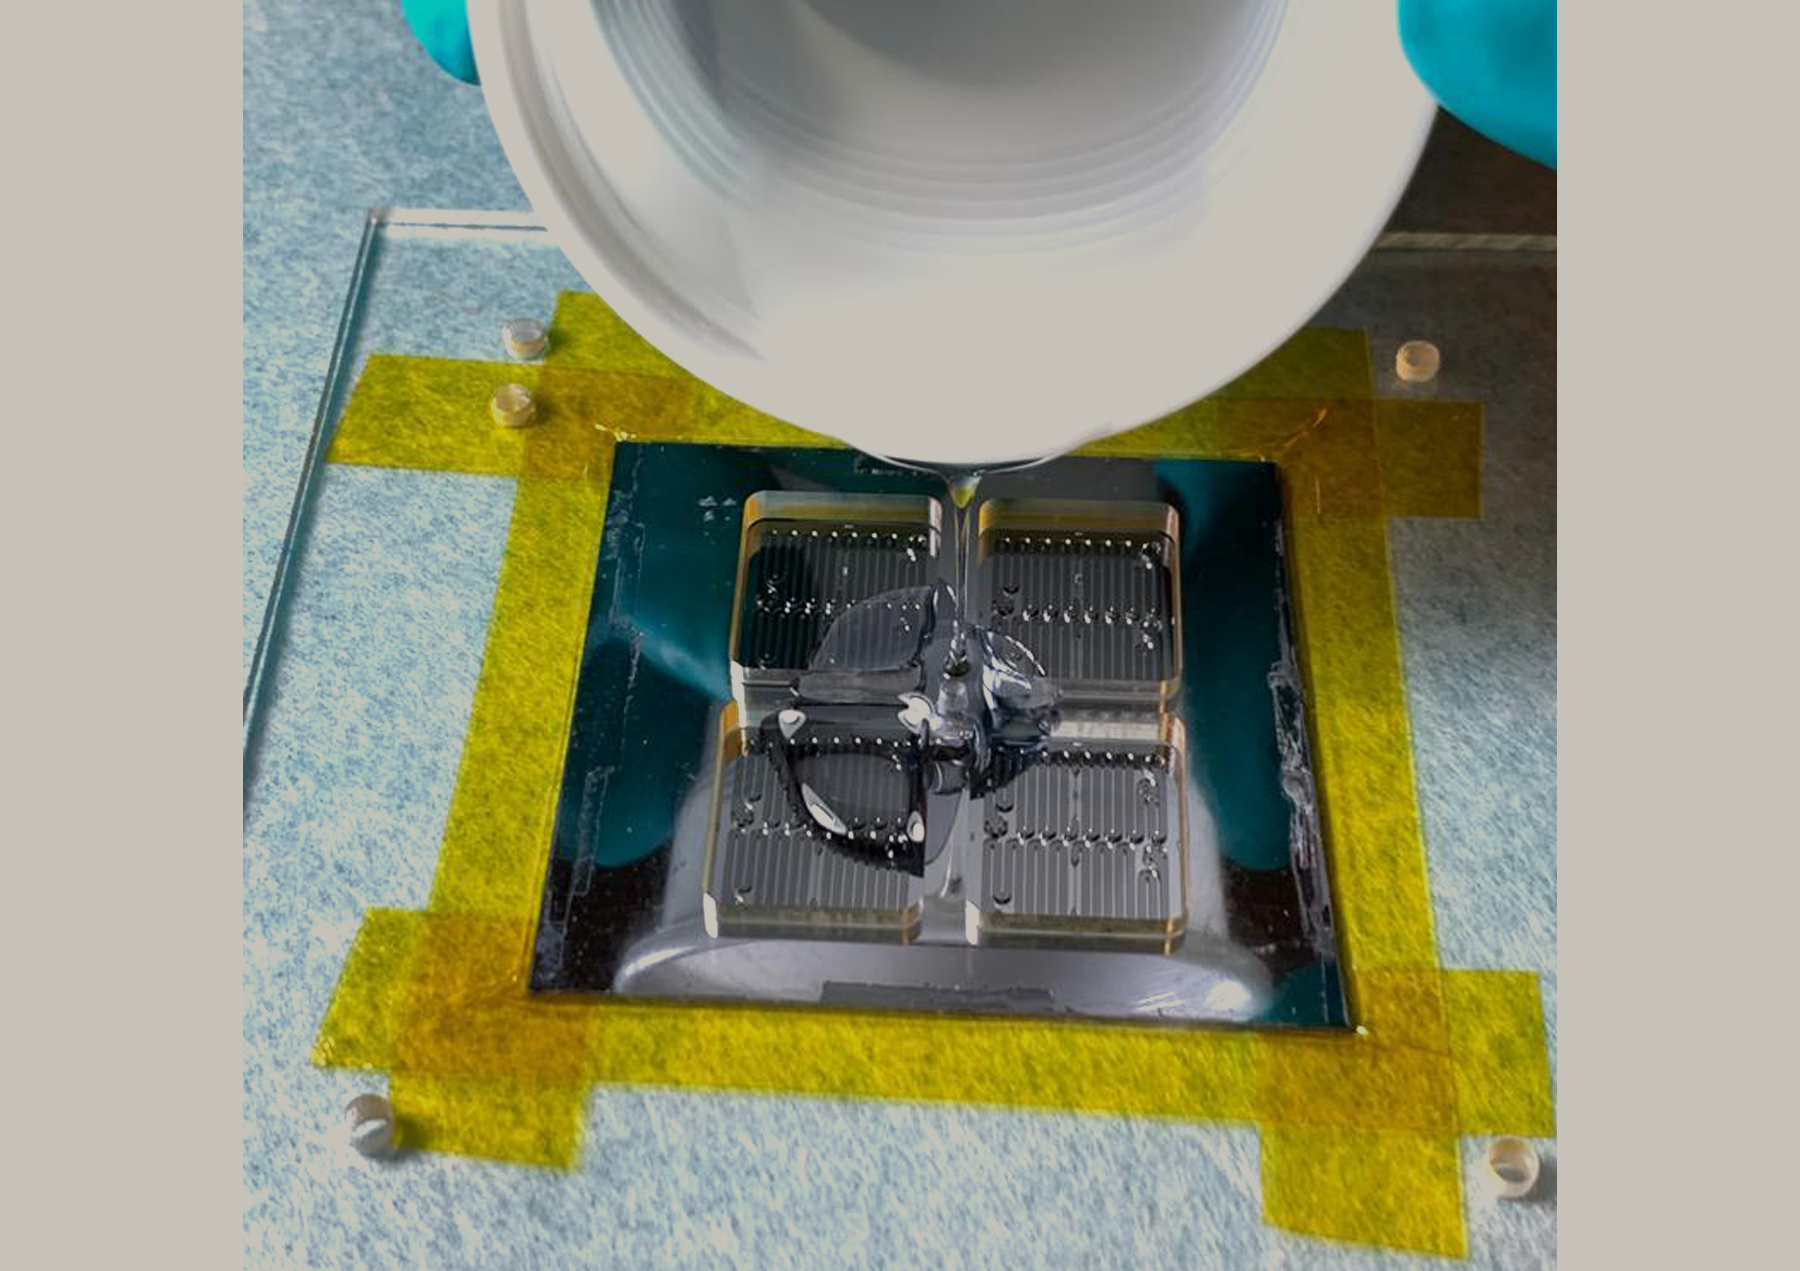
\includegraphics[width=\linewidth]{images/appendix_b/pour.png}
        \caption{PDMS pouring into the mold.}
        \label{figure:pdms-pouring}
    \end{subfigure}

    \caption{Microfluidic channel fabrication process.}
    \label{figure:pdms}
\end{figure}

During my internship, I collaborated closely with Eng. Ruben Afonso and Eng. Beatriz Borges. When I joined the project, the hard-mask (Figure \ref{figure:pdms-hardmask}) responsible for defining the format of the microfluidic channel, through which the samples flow, had already been fabricated. Therefore, my involvement mainly focused on the fabrication of the \ac{PDMS} material and the channels themselves. The \ac{PDMS} serves as the structural component of the channels. One specific channel (Figure \ref{figure:pdms-mask}) design that Eng. Ruben Afonso wanted to test was the incorporation of a serpentine shape. The objective behind this unique design was to maximize the utilization of space within the sensor chip for storing the samples to be analyzed. The serpentine shape functions like a reservoir, enabling the samples to pass through the extremely narrow central channel multiple times. This repeated passage through the channel, where the sensors are located, allows for redundant measurements, ultimately enhancing the reliability and accuracy of the results. In addition to the hard-mask, an acrylic mold (Figure \ref{figure:pdms-mold}) was also a necessary component for the fabrication process. While the hard-mask defines the shape of the microfluidic channel, the acrylic mold is responsible for shaping the \ac{PDMS} material. The acrylic mold was precisely cut at \ac{INESC-MN} and required careful alignment with the hard-mask to ensure accurate replication. Once the alignment was achieved, the \ac{PDMS} preparation was poured into the mold, Figure \ref{figure:pdms-pouring}. It is essential to shape the inlets and outlets of the channels using tubes that allow the insertion of samples. Afterward, the \ac{PDMS} preparation is cured, and the microfluidic channels are ready to be extracted.

\begin{figure}[!ht]
    \centering
    \begin{subfigure}[b]{.475\linewidth}
        \centering
        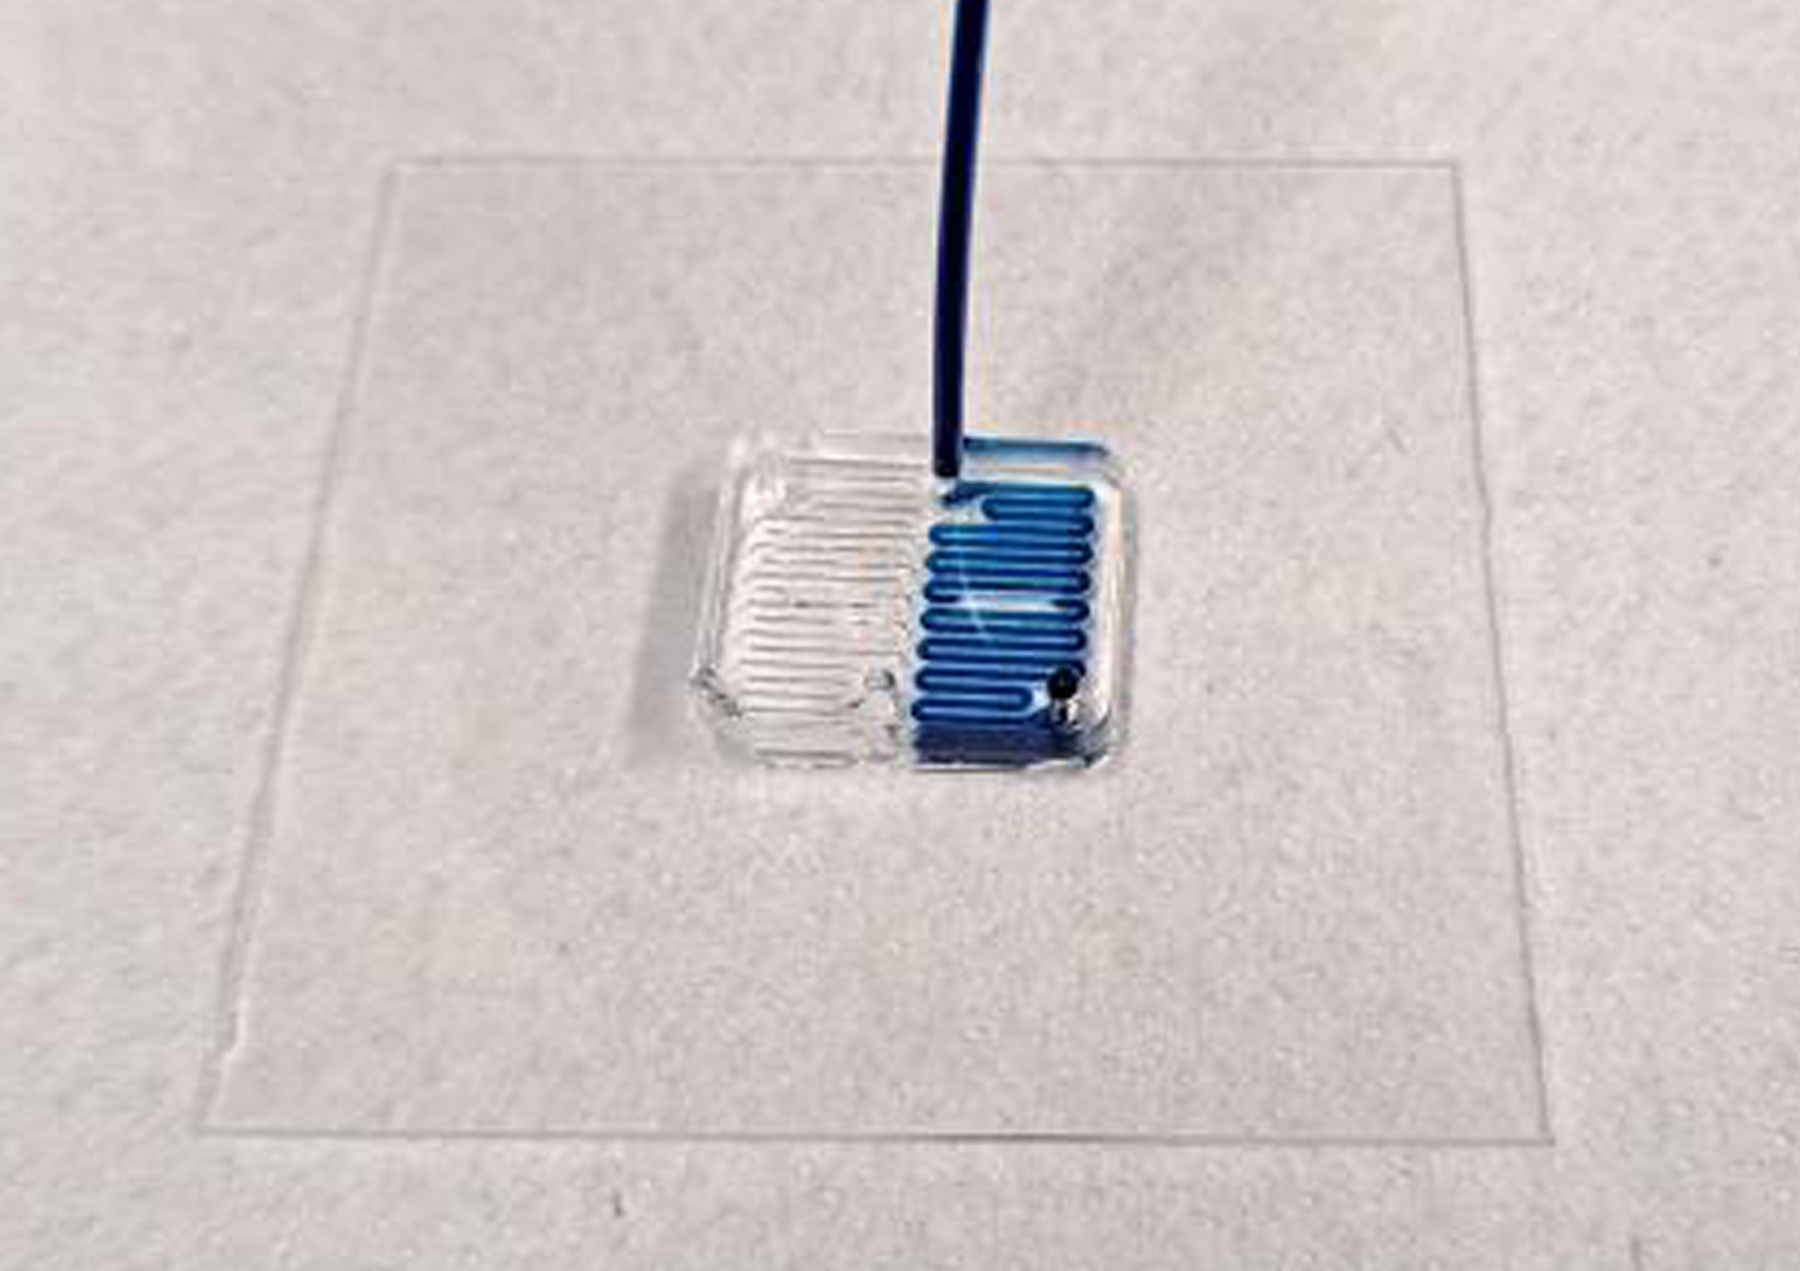
\includegraphics[width=\linewidth]{images/appendix_b/test.png}
        \caption{Testing of the PDMS channels.}
        \label{figure:mf-test}
    \end{subfigure}
    \hfill
    \centering
    \begin{subfigure}[b]{.475\linewidth}
        \centering
        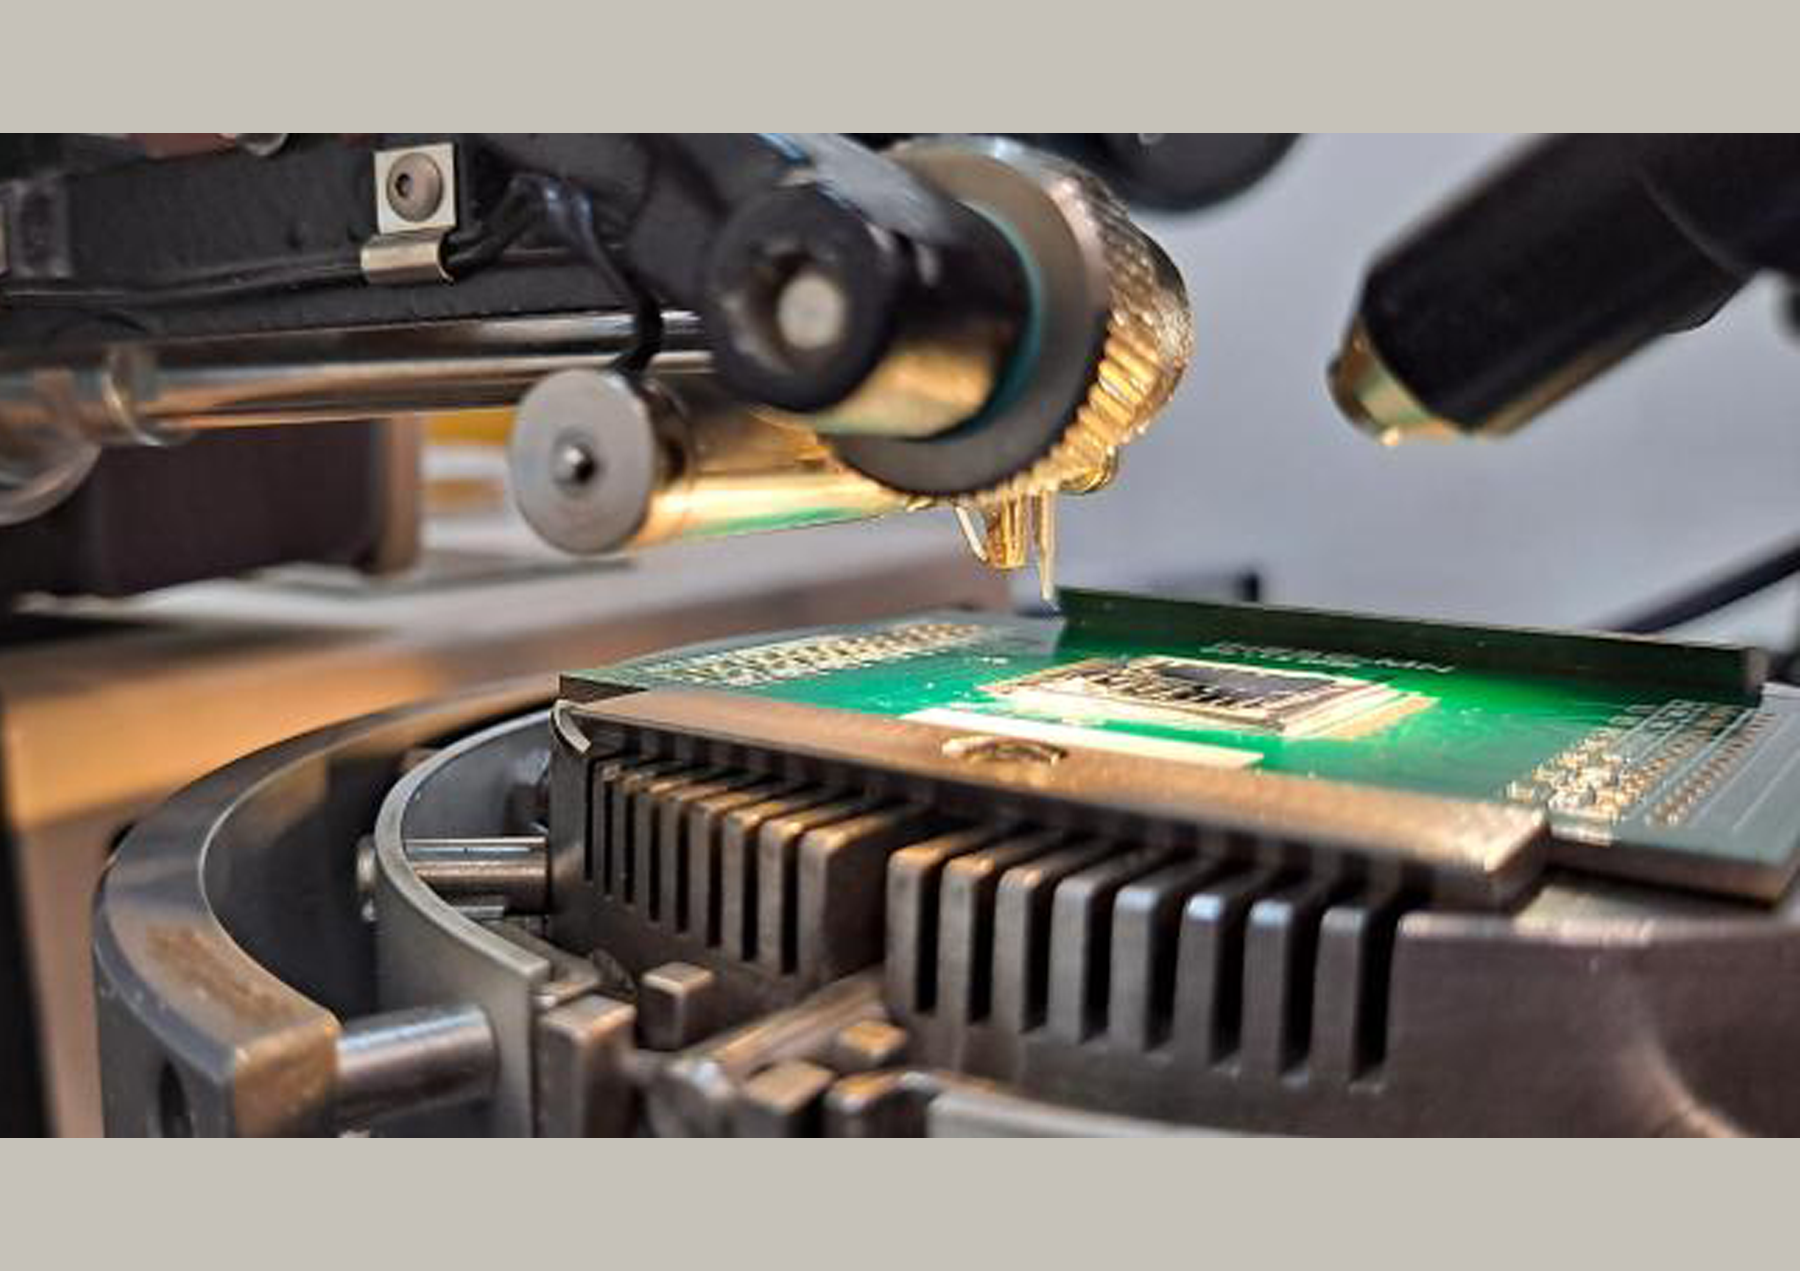
\includegraphics[width=\linewidth]{images/appendix_b/wirebonding.png}
        \caption{Wire-Bonding -- Sensor chip to PCB.}
        \label{figure:mf-wbonding}
    \end{subfigure}

    \bigskip
    
    \centering
    \begin{subfigure}[b]{.475\linewidth}
        \centering
        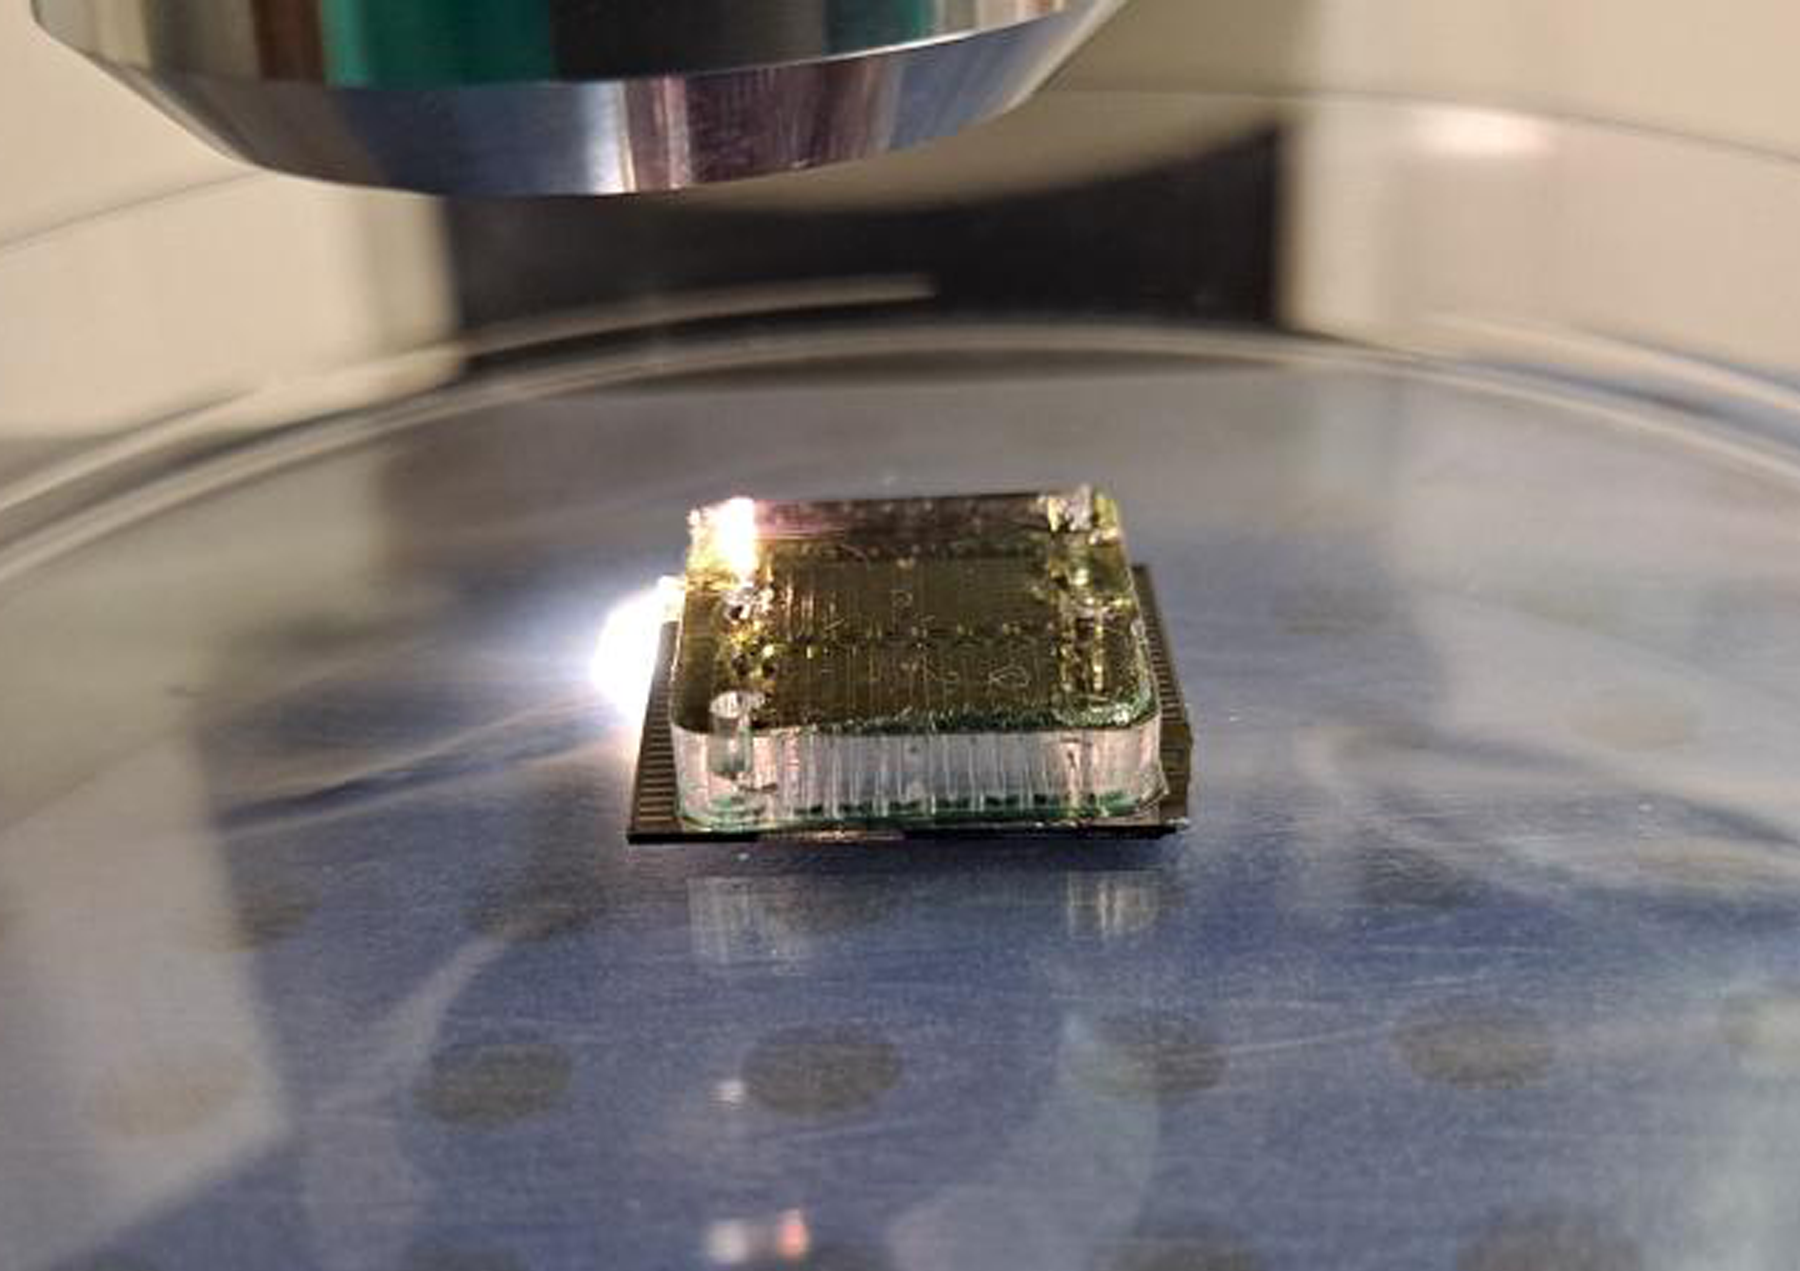
\includegraphics[width=\linewidth]{images/appendix_b/bonding.png}
        \caption{Bonding -- Microfluidic channel to sensor chip.}
        \label{figure:mf-bonding}
    \end{subfigure}
    \hfill
    \centering
    \begin{subfigure}[b]{.475\linewidth}
        \centering
        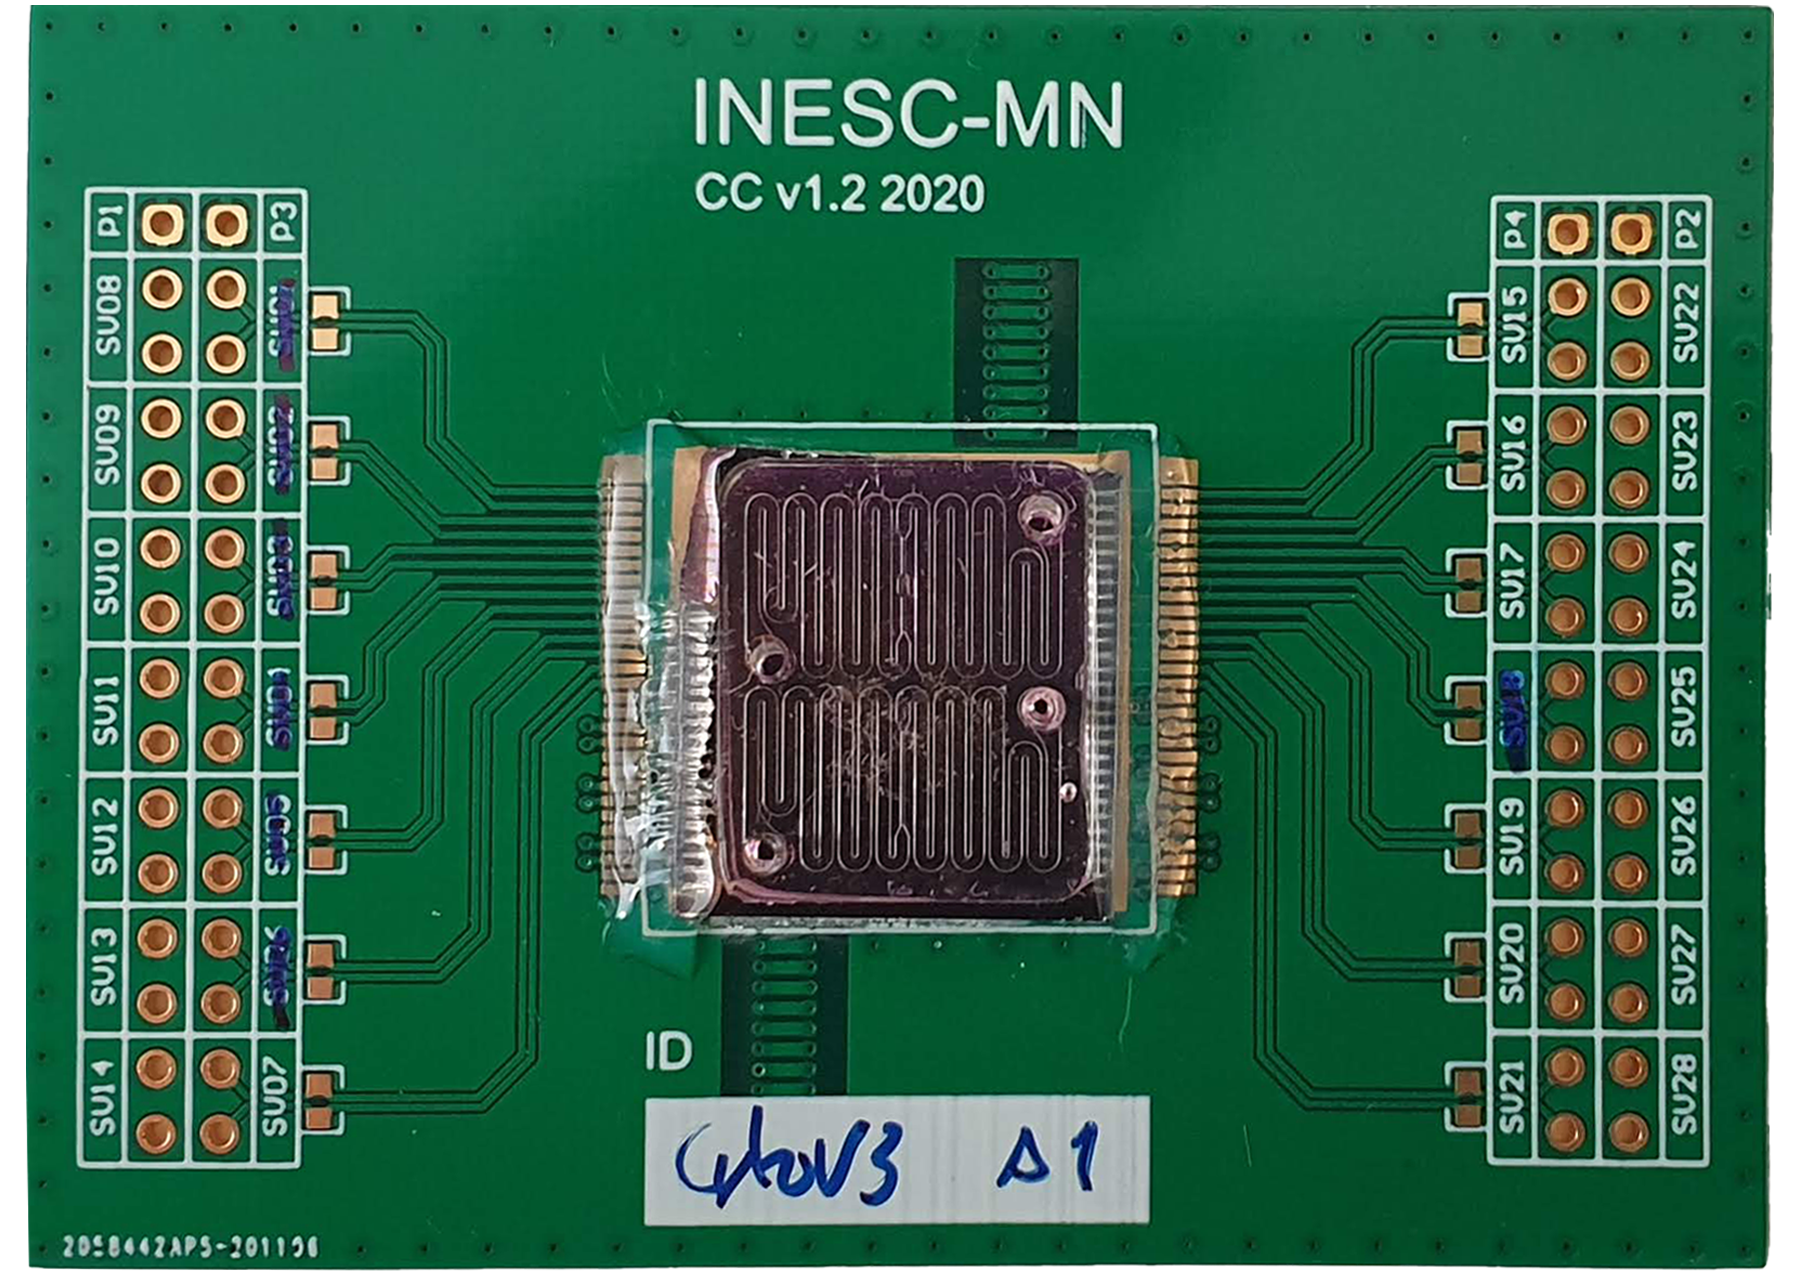
\includegraphics[width=\linewidth]{images/appendix_b/sensorpcb_b.png}
        \caption{Result -- PCB, MR sensors and microfluidic channels.}
        \label{figure:mf-result}
    \end{subfigure}

    \caption{Microfluidic channel integration in the system.}
    \label{figure:microfluidic}
\end{figure}

After the fabrication of the \ac{PDMS} microfluidic channels, the batch undergoes testing (Figure \ref{figure:mf-test}) using a sample composed of water and food coloring. This test aims to ensure that the channels are not clogged. The channels are bonded to a glass substrate for this purpose. Once the batch passes the testing phase successfully, the microfluidic channels are ready to be bonded to a sensor chip (Figure \ref{figure:mf-bonding}) that has been wire-bonded (Figure \ref{figure:mf-wbonding}) onto the \ac{PCB} beforehand. The resulting assembly, depicted in Figure \ref{figure:mf-result}, is then ready to be integrated with the interface developed in this work.

\clearpage
\thispagestyle{empty}
\cleardoublepage
